\documentclass[a4 paper]{article}
\usepackage[inner=2.0cm,outer=2.0cm,top=2.5cm,bottom=2.5cm]{geometry}
\usepackage{setspace}
\usepackage{graphics}
\usepackage[rgb]{xcolor}
\usepackage{verbatim}
\usepackage{subcaption}
\usepackage{amsgen,amsmath,amstext,amsbsy,amsopn,tikz,amssymb}
\usepackage{fancyhdr}
\usepackage[colorlinks=true, urlcolor=blue,  linkcolor=blue, citecolor=blue]{hyperref}
\usepackage[colorinlistoftodos]{todonotes}
\usepackage{rotating}
\usepackage{booktabs}
\newcommand{\ra}[1]{\renewcommand{\arraystretch}{#1}}

\newtheorem{thm}{Theorem}[section]
\newtheorem{prop}[thm]{Proposition}
\newtheorem{lem}[thm]{Lemma}
\newtheorem{cor}[thm]{Corollary}
\newtheorem{defn}[thm]{Definition}
\newtheorem{rem}[thm]{Remark}
\numberwithin{equation}{section}

\newcommand{\homework}[6]{
   \pagestyle{myheadings}
   \thispagestyle{plain}
   \newpage
   \setcounter{page}{1}
   \noindent
   \begin{center}
   \framebox{
      \vbox{\vspace{2mm}
    \hbox to 6.28in { {\bf CSE 211:~Discrete Mathematics \hfill {\small (#2)}} }
       \vspace{6mm}
       \hbox to 6.28in { {\Large \hfill #1  \hfill} }
       \vspace{6mm}
       \hbox to 6.28in { {\it Instructor: {\rm #3} \hfill  {\rm #5} \hfill  {\rm #6}} \hfill}
       \hbox to 6.28in { {\it Assistant: #4  \hfill #6}}
      \vspace{2mm}}
   }
   \end{center}
   \markboth{#5 -- #1}{#5 -- #1}
   \vspace*{4mm}
}

\newcommand{\problem}[2]{~\\\fbox{\textbf{Problem #1}}\hfill (#2 points)\newline\newline}
\newcommand{\subproblem}[1]{~\newline\textbf{(#1)}}
\newcommand{\D}{\mathcal{D}}
\newcommand{\Hy}{\mathcal{H}}
\newcommand{\VS}{\textrm{VS}}
\newcommand{\solution}{~\newline\textbf{\textit{(Solution)}} }


\newcommand{\bbF}{\mathbb{F}}
\newcommand{\bbX}{\mathbb{X}}
\newcommand{\bI}{\mathbf{I}}
\newcommand{\bX}{\mathbf{X}}
\newcommand{\bY}{\mathbf{Y}}
\newcommand{\bepsilon}{\boldsymbol{\epsilon}}
\newcommand{\balpha}{\boldsymbol{\alpha}}
\newcommand{\bbeta}{\boldsymbol{\beta}}
\newcommand{\0}{\mathbf{0}}


\begin{document}

\homework{Homework \#2}{Due: 07/12/20}{Dr. Zafeirakis Zafeirakopoulos}{Gizem S\"ung\"u}{}{}


\problem{1: Relations}{15}
Draw the Hasse diagram for the “greater than or equal to” relation on $\{$0, 1, 2, 3, 4, 5$\}$.

\solution
To draw a Hasse diagram, provided set must be a poset.
A poset or partially ordered set A is a pair, ( B, $\leq$ ) of a set B whose elements are called the vertices of A and
obeys following rules:
\begin{itemize}
    \item Reflexivity : p  $\leq$  p $\forall$ p $\in$ B.
    \item Anti-symmetric : p $\leq$ q and q $\geq$ p iff p = q.
    \item Transitivity : if p $\leq$ q and q $\leq$ r then p $\leq$ r.
\end{itemize}
We have to find the poset for the greater than or equal to. "$\geq$ " says "a relation (a, b) where a, b $\in$  B, a is greater than or equal to b."
\newline
\newline
Let the set is A. Then,
A = \{(0 $\prec$ 0), (1 $\prec$ 1), (2 $\prec$ 2), (3 $\prec$ 3), (4 $\prec$ 4), (5 $\prec$ 5), (5 $\prec$ 4), (5 $\prec$ 3), (5 $\prec$ 2), (5 $\prec$ 1), (5 $\prec$ 0), (4 $\prec$ 3), (4 $\prec$ 2), (4 $\prec$ 1), (4 $\prec$ 0), (3 $\prec$ 2), (3 $\prec$ 1), (3$\prec$ 0),  (2 $\prec$ 1), (2$\prec$ 0), (1 $\prec$ 0)\}
Let's draw the directed graph the relation above in Figure 1:
\begin{figure}[h!]
  \centering
  \begin{subfigure}[b]{0.4\linewidth}
    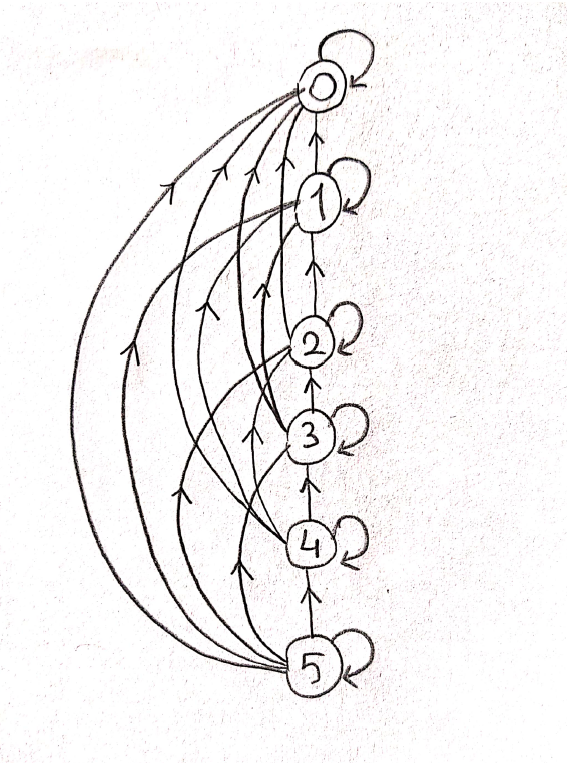
\includegraphics[width=\linewidth]{fig1.png}
    \caption{Figure 1:The original graph}
  \end{subfigure}
\end{figure}
\newpage
Since we know that a poset MUST provide reflexivity, we also do not need the reflexive relations in A.Hence A can be updated as:
A = \{(5 $\prec$ 4), (5 $\prec$ 3), (5 $\prec$ 2), (5 $\prec$ 1), (5 $\prec$ 0), (4 $\prec$ 3), (4 $\prec$ 2), (4 $\prec$ 1), (4 $\prec$ 0), (3 $\prec$ 2), (3 $\prec$ 1), (3$\prec$ 0),  (2 $\prec$ 1), (2$\prec$ 0), (1 $\prec$ 0)\}
\newline
In the next step, remove the self-loops in Figure 2:
\begin{figure}[h!]
  \centering
  \begin{subfigure}[b]{0.4\linewidth}
    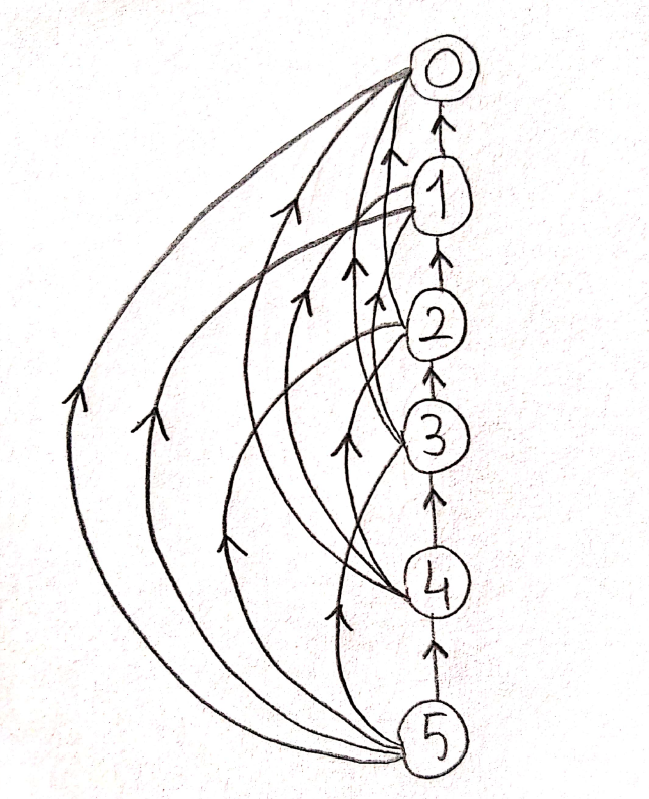
\includegraphics[width=\linewidth]{fig2.png}
    \caption{Figure 2:The graph without self-loops}
  \end{subfigure}
\end{figure}
\newline\newline
Remove the transivite edges and the hasse diagram is obtained in Figure 3:
\begin{figure}[h!]
  \centering
  \begin{subfigure}[b]{0.2\linewidth}
    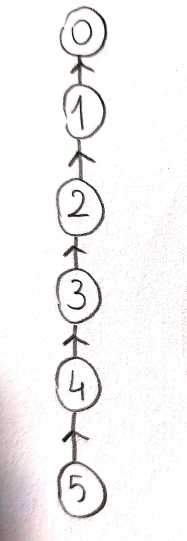
\includegraphics[width=\linewidth]{fig3.png}
    \caption{Figure 3:The Hasse diagram}
  \end{subfigure}
\end{figure}

\newpage

\problem{2: Relations}{15}
Answer these questions for the poset ($\{\{$1$\}$, $\{$2$\}$, $\{$4$\}$, $\{$1, 2$\}$, $\{$1, 4$\}$, $\{$2, 4$\}$, $\{$3, 4$\}$, $\{$1, 3, 4$\}$, $\{$2, 3, 4$\}\}$, $\subseteq$).
\newline
\subproblem{a} Find the maximal elements.
\solution
In a Hasse diagram, a vertex corresponds to a maximal element if there is no edge leaving the vertex.
In Figure 4, $\{$1, 2$\}$, $\{$1, 3, 4$\}$ and $\{$2, 3, 4$\}$ are the maximal elements because there are no edge leaving these verticies.
\newline
\subproblem{b} Find the minimal elements.
\solution
In a Hasse diagram, a vertex corresponds to a minimal element if there is no edge entering the vertex.
In Figure 4, $\{$1$\}$, $\{$2$\}$ and $\{$4$\}$ are the minimal elements because there are no edge entering these verticies.
\newline
\subproblem{c} Is there a greatest element?
\solution
An element is called the greatest element if it is greater than every other element of the poset. In Figure 4, the greatest element does not exist since there is no any one element that succeeds all the elements.
\newline
\subproblem{d} Find all upper bounds of $\{\{$2$\}$, $\{$4$\}\}$.
\solution
Let B be a subset of a poset A. An element x $\in$ A is called an upper bound of B if y $\leq$ x for every y $\in$ B.
In Figure 4, $\{$2, 4$\}$ and $\{$2, 3, 4$\}$ are upper bounds of $\{\{$2$\}$,$\{$4$\}\}$ because \{$2$\}$\leq$$\{$2, 4$\}$ , \{$4$\}$\leq$$\{$2, 4$\}$ and \newline \{$2$\}$\leq$$\{$2, 3, 4$\}$, \{$4$\}$\leq$$\{$2, 3, 4$\}$ .
\newline
\subproblem{e} Find the least upper bound of $\{\{$2$\}$, $\{$4$\}\}$, if it exists.
\solution
The element x is called the least upper bound of the subset A if x is an upper bound that
is less than every other upper bound of A.In Figure 4, $\{$2, 4$\}$ is the least upper bound of $\{\{$2$\}$,$\{$4$\}\}$ .

\subproblem{f} Find all lower bounds of $\{\{$1, 3, 4$\}$, $\{$2, 3, 4$\}\}$.
\solution
Let B be a subset of a poset A. An element z $\in$ A is called a lower bound of B if z $\leq$ x for every x $\in$ B. In Figure 4, $\{$3, 4$\}$, $\{$3$\}$ and $\{$4$\}$ are lower bounds of $\{\{$1, 3, 4$\}$, $\{$2, 3, 4$\}\}$ because $\{$3, 4$\}$ $\leq$ $\{$1, 3, 4$\}$, $\{$3$\}$ $\leq$ $\{$1, 3, 4$\}$,  $\{$4$\}$ $\leq$ $\{$1, 3, 4$\}$ and $\{$3, 4$\}$ $\leq$ $\{$2, 3, 4$\}$, $\{$3$\}$ $\leq$ $\{$2, 3, 4$\}$,  $\{$4$\}$ $\leq$ $\{$2, 3, 4$\}$ .

\subproblem{h} Find the greatest lower bound of $\{\{$1, 3, 4$\}$, $\{$2, 3, 4$\}\}$,
if it exists.
\solution
The element x is called the greatest lower bound of the subset A if x is an lower bound that is greater than every other lower bound of A.
In Figure 4, $\{$3, 4$\}$is the greatest lower bound of $\{\{$1, 3, 4$\}$, $\{$2, 3, 4$\}\}$.
\begin{figure}[h!]
  \centering
  \begin{subfigure}[b]{0.4\linewidth}
    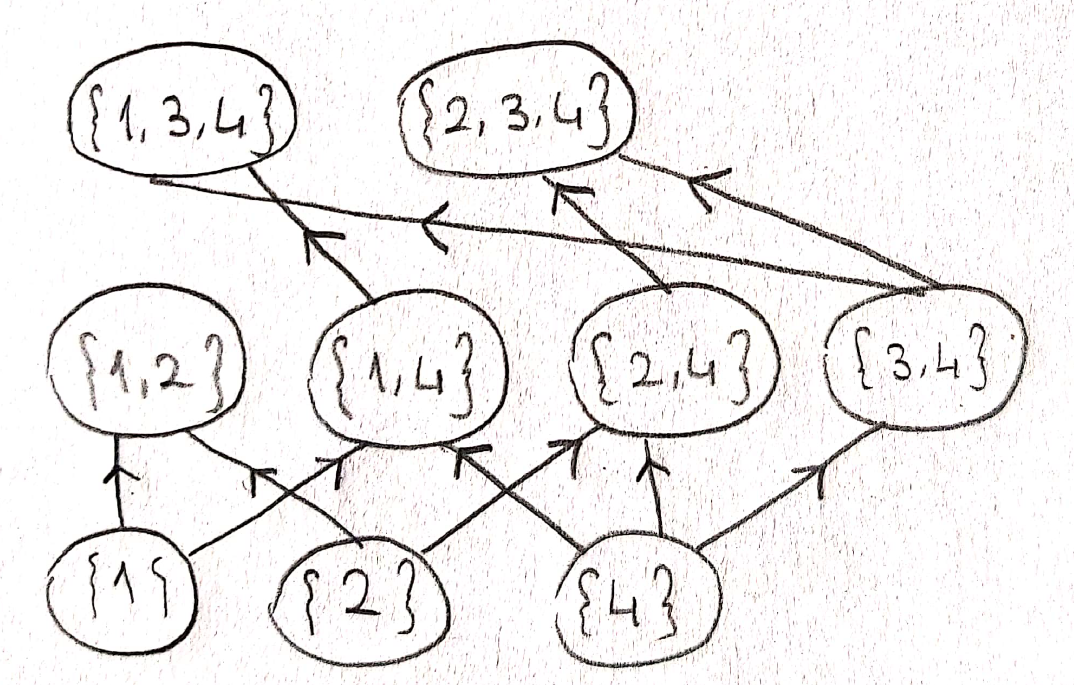
\includegraphics[width=\linewidth]{fig4.png}
    \caption{Figure 4}
  \end{subfigure}
\end{figure}
\newpage
\problem{3: Relations}{70}
Remember that a relation $R$ on a set $A$ can have the properties reflexive, symmetric, anti-symmetric and transitive.

\begin{itemize}
	\item $\textbf{Reflexive: }$ R is reflexive if (a, a) $\in$ $R$, $\forall$ a $\in$ A.
	\item $\textbf{Symmetric: }$ R is symmetric if (b, a) $\in$ R whenever (a, b) $\in$ R, $\forall$ a, b $\in$ A.
	\item $\textbf{Anti-symmetric: }$ R is antisymmetric if $\forall$ a, b $\in$ A, (a, b) $\in$ R and (b, a) $\in$ R implies that a = b.
	\item $\textbf{Transitive: }$ R is transitive if $\forall$ a, b, c $\in$ A, (a, b) $\in$ R and (b, c) $\in$ R implies that (a, c) $\in$ R.
\end{itemize}
For the details about the properties, please check the 4th lecture slide on Moodle. \\

As we solved the problem 3 in PS4 document - which is available on Moodle - in the problem session, we can determine any given relation if it is reflexive, symmetric, anti-symmetric, and transitive.\\

Write an algorithm to determine if a given relation $R$ is reflexive, symmetric, anti-symmetric, and transitive. Your code should meet the following requirements, standards and tasks.

\begin{itemize}
	\item Read the relations in the text file "input.txt".
	\item Let $R$ be a relation on a set $A$ where $\exists a,b \in A, (a,b) \in R$. Each relation $R$ is represented with 3 lines in the file:
	\begin{itemize}
		\item [1.] The first line says how many relations in $R$.
		\item[2.] The second line gives the elements of the set $A$.
		\item[3.] The following lines gives each relation in $R$.
	\end{itemize}
	\item After determining each relation in input.txt whether it is reflexive, symmetric, anti-symmetric and transitive with your algorithm, write its result to the file which is called "output.txt" with the following format.
	\item output.txt:
	\begin{itemize}
		\item[1.] Start a new line with "n" which indicates a new relation.
		\item[2.] The set of $R$
		\item[3.] Reflexive: Yes or No, explain the reason if No (e.g. "(a, a) is not found").
		\item[4.] Symmetric: Yes or No, explain the reason if No (e.g. "(b, a) is not found whereas (a, b) is found.")
		\item[5.] Antisymmetric: Yes or No, explain the reason if No (e.g. "(b, a) and (a, b) are found.")
		\item[6.] Transitive: Yes or No, explain the reason if No (e.g. "(a, c) is not found whereas (a, b) and (b, c) are found.")
	\end{itemize}
	\item An example of the output format is given in "exampleoutput.txt". The file has the result of the first relation in "input.txt".
	\item When explaining why a property does not exist in the relation, one reason is enough to explain if there are more. For example, in "exampleoutput.txt", the relation is not symmetric because (b, a) and (e, a) are not found. Detecting one of them is enough to explain the reason.
	\item $\textbf{Bonus (20 points): }$ If you can explain why a property exists in the relation, it brings you bonus of 20 points.
	\item Your code is responsible to provide exception and error handling. The input file may be given with a wrong information, then your code must be prepared to detect them. For instance, "The element b of the relation (1, b) is not found in the set A = $\{1, 2, 3, 4\}$.".
	\item You can implement your algorithm in Python, Java, C or C++.
	\item $\textbf{Important: }$ Put comments almost for each line of your code to describe what the line is going to do. 
	\item You should put your source code file (file name is problem1.$\{.c, .java, .py, .cpp\}$) and output.txt into your homework zip file (check Course Policy).
\end{itemize}



\end{document} 
